\chapter{Post Mortem I}

\textbf{Recap}\\
The trouble with the target matrix in the last example is that it does not have enough linearly independent column vectors to span the domain. For this reason, the matrix does not have a left inverse. Also, a \textit{separate} issue is the lack of linearly independent row vectors to span the codomain. This explains why there is no right inverse. Therefore the linear system can't be solved using obvious methods. Hence the need for the SVD and the pseudoinverse.

The principle of organization for the last two and subsequent chapters is that matrices are collections of row vectors and collection of column vectors. 
\begin{equation}
  \A{}=\Aexample = \underbrace{\mat{c|c}{c_{1} & -c_{1}}}_{\text{image of }\A{}}=\underbrace{\mat{r}{r_{1}^{\mathrm{T}}\\\hline-r_{1}^{\mathrm{T}}\\\hline r_{1}^{\mathrm{T}}}}_{\text{image of }\A{T}}
\end{equation}
with the linearly independent vectors having the assignments
\begin{equation}
  c_{1}=\mat{r}{1\\-1\\1}, \quad r_{1}=\mat{r}{1\\-1}.
\end{equation}
The nettlesome issue is that neither image covers the induced matrix spaces of $\real{2}$ and $\real{3}$:
\begin{equation}
  \spn\lst{\mat{r}{1\\-1\\1}}=\real{1}\ne\real{3}, \qquad \spn\lst{\mat{r}{1\\-1}}=\real{1}\ne\real{2}.
\end{equation}

The \svdl \ explicitly separated domain and codomain into two matrices $\X{}$ and $\Y{}$. These matrices resolve the two domains into complete orthonormal spaces for $\real{m=2}$ (domain) and $\real{n=3}$ (codomain).
 
We start with a matrix whose dimension dictates the dimensions of the domains. This separation splits the row and vector spaces apart leaving four fundamental components. For the \vv \ world of the domain they are these:
\begin{enumerate}
\item an orthonormal span of the linearly independent \textit{row} vectors; also called the image space of $\A{}$,
\item an orthonormal span of the perpendicular complement, $\null{\A{}}$; also call the kernel.
\end{enumerate}
For the \vvv \ world of the codomain we have these:
\begin{enumerate}
\item an orthonormal span of the linearly independent \textit{column} vectors; also called image space of $\A{T}$,
\item an orthonormal span of the perpendicular complement, $\null{\A{T}}$; also call the cokernel.
\end{enumerate}
The diagram in figure \eqref{fig:pm:decomp} shows these relationships in abbreviated form.

\begin{figure}[htbp] %  figure placement: here, top, bottom, or page
   \centering
   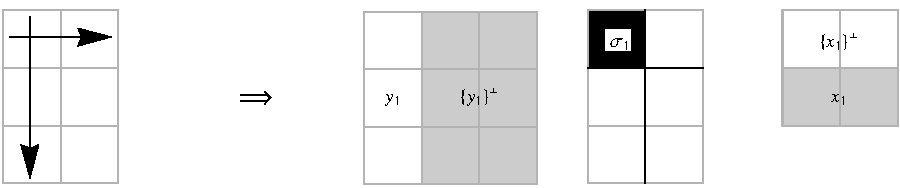
\includegraphics[ width = 5in ]{pdf/post_mortem/earlydecomp.pdf} 
   \caption{A schematic look at the \svdl. In the previous chapter we took a matrix with one linearly independent column vector (down arrow) and one linearly independent row vector (right arrow) and resolved the domain and codomain into four fundamental subspaces shown here.}
   \label{fig:pm:decomp}
\end{figure}

\textbf{Quo vadis?}\\
This chapter will look at the result in a bit more detail. In particular focus will be drawn to which of this spaces are the physical space of measurements and which are the abstract aphysical spaces of the fit parameters.

The last chapter presented a least squares solution using \textit{orthogonal projection}\index{orthogonal projection} to minimize the distance between the measurement vector and the range of the target matrix. Here we connect this result with solution to the normal equations.

%%
\section{Interpretation of the system}
We saw that the linear system in equation \eqref{eq:2:problem} has no solution. There is no possible vector $\xi$ such that
\begin{equation}
  \A{}\xi=\phi.
\end{equation}
Yet we have answer, we found a value for the vector $\xi$. What is the significance of this $2-$vector? Under the mapping action $\A{}$, the $2-$vector in the domain corresponds to the $3-$vector $p=\A{}\xi$ in the codomain. The solution we have constructed minimizes the distance between the data $\phi$ and the image of $\A{}$. 

Put another way, the vector $\xi$ which minimizes the error norm
\begin{equation}
  \normt{\epsilon}^{2} = \normt{\A{}\xi-\phi}^{2}.
\end{equation}
is the orthogonal projection of the data onto the range of $\A{}$. Notice that the minimization occurred in the codomain. The next part of the problem involves the inverse problem: connecting this closest point in the codomain to a point in the domain.

%%
\subsection{The special solution}
We see that the special solution provided by the pseudoinverse,
\begin{equation}
  \A{+}\phi = \xi_{p}
\end{equation}
is the particular solution. The \vvv 
\begin{equation*}
  \A{}\xi_{p} = p
\end{equation*}
is the orthogonal projection of the data onto the range or $\A{}$ and as such is the solution with the minimum $2-$norm.

In some sense, all roads lead to Rome and we could have obtained this same solution using the normal equations, calculus or numerical iteration. The advantage of using the SVD is that we see a clear decomposition of the ranges and null spaces which we can use to visualize the geometry and quality of the solutions. Let's explore these other solution methods.

%%
\subsection{The merit function in parameter space}
In a classic least squares fit, one minimizes a merit function to find the solution. This merit function quantifies the difference between each measurement and the prediction. These differences are called the residual errors. The method of least squares minimizes the sums of the squares of these residual errors. A candidate merit function is
\begin{equation}
  M(\xi) = \normt{\A{}\xi-\phi}^{2} = \paren{\A{}\xi-\phi}^{\mathrm{T}}\paren{\A{}\xi-\phi}.
  \label{eq:merit}
\end{equation}

The plots below show what this merit function looks like. Observe that the merit function takes a $2-$vector as the argument and returns a scalar, a real number. These figures show the solution and how the merit function changes under perturbations of the input variables. The problem with plotting the merit function is seen in the figure. All solutions along the dashed line have the same value for the merit function. Without knowledge of the range of the target matrix we are unable to select any one answer.

\begin{figure}[t] %  figure placement: here, top, bottom, or page
   \centering
   \includegraphics[ width = 3.25in ]{pdf/post_mortem/threed} \\[10pt]
   \includegraphics[ width = 3.25in ]{pdf/post_mortem/contour}
   \caption[Equivalent views of the merit function in parameter space]{Equivalent views of the merit function in parameter space: the domain. The figure on the top is a 3D rendering which reveals the basic shape of the error hypersurface. The contour plot on the bottom is more useful for qualitative analysis. This plot shows the solution $\A{+}\phi$ (white point) and the space resolved into orthogonal coordinates, the image space  $\X{}_{:,1}$ (dashed line) and the null space $\X{}_{:,2}$ (faint dotted line). The merit function does not have a minimum point; the locus of minima is line which defines the null space. space, the dashed line. The intersection of the range space and the minima is the particular solution.}
   \label{fig:2:merit}
\end{figure}
\clearpage


The SVD warned us that we could only minimize the merit function along a line: there was a solitary singular value. The zero eigenvalues signal that the system is inconsistent or underdetermined.

%%s
\section{Solution using the calculus}
The particular solution also comes from a basic calculus problem: minimize the distance between a point and a line. The point is the measurement and the line is the span of the image vector. Of course a concern is that we are not solving the problem with these machinations. We are finding a \vvv \ in the image; we need the \vv \ in domain that maps to this \vvv.

The line represents the fundamental column in $\A{}$ and is parameterized as
\begin{equation}
  \begin{split}
    f(\alpha)=\alpha\mat{r}{1\\-1\\1}.
    \label{eq:range}
  \end{split}
\end{equation}
The square of the $L_{2}$ distance $d_{2}$ between the data and the image is given by
\begin{equation}
  d_{2}^{2}\paren{\phi,f(\alpha)} = \normt{\phivector-\mat{r}{\alpha\\-\alpha\\ \alpha}}^{2} = 3\alpha^{2}-2\alpha+5.
\end{equation}
Minimize this distance in the canonical fashion: set the first derivative equal to zero and solve for $\alpha$. The result is this
\begin{equation}
  \alpha = \frac{1}{3}.
\end{equation}
This implies that the point $p$ on the line $f(\alpha)$ closest to the data point is this
\begin{equation}
  p=\frac{1}{3}\mat{r}{1\\-1\\1}.
  \label{eq:p}
\end{equation}
\begin{figure}[h]
   \centering
   \includegraphics[ ]{pdf/simple/image03.pdf} 
   \caption[The picture in the space of measurements]{The picture in the space of measurements: the image. The thick black line is the range $\rng{\A{}}$ or image of the matrix $\A{}$ given by equation \eqref{eq:range}. The blue arrow represents the measurement vector $\phi$ in equation \eqref{eq:phi}. The least squares solution is the orthogonal projection (red arrow) from the data vector onto the image of the row space. The solution point on the image is also in red and is given in equation \eqref{eq:p}. All of these constructs are shadowed on the floor to help with the perspective. The \vvv \ $p$ is not the solution. The final answer is the \vv \ $\xi_{p}$ which maps to $p$ via $\A{}\xi_{p}=p$. }
   \label{fig:image}
\end{figure}

Notice that the point $p$ is a \vvv \ and therefore a resident of the codomain. The solution must be a \vv \ from the domain. The question now arises: which \vv \ $\xi_{p}$ in the domain connects to the \vvv \ $p$? Mathematically we are solving this equation for $\xi_{p}$:
\begin{equation}
  \A{}\xi_{p}=p.
\end{equation}

Before you lament that we have gone back to the beginning and are solving the same linear system observe that this time there is an exact solution. The data vector $p$ is in the image of  the system matrix $\A{}$. 

Because the system is basic we guess the solution to the equation
\begin{equation}
 \Aexample \mat{c}{\xi\\\eta} = \frac{1}{3}\mat{r}{1\\-1\\1}
\end{equation}
is given by
\begin{equation}
  \mat{c}{\xi\\\eta}=\frac{1}{6}\mat{r}{1\\-1}.
\end{equation}

What if the problem is more complicated? In the case of the normal equations we can depend upon an elimination scheme to provide the solution.

\endinput
\section[The bounty from the SVD]{The bounty from \svdl}
The elegance of the SVD blossoms when we examine the domain and the codomain in terms of contributions from the target matrix to the $\X{}$ and $\Y{}$ matrices shown in table \eqref{tab:vecs}.

\subsection{The row space: home of the solution}
The domain is $\real{2}$ and is resolved into two orthonormal vectors. The first vector comes from the first row vector (the first column in the matrix transpose) and becomes  $\X{}_{*,1}$. The orthogonal complement is \textit{constructed} based upon the first vector. The result becomes $\X{}_{*,2}$.

\subsection{The column space: home of the measurements}
The codomain is $\real{3}$ and requires three orthonormal vectors. The first vector comes from the first column vector in the target matrix and becomes  $\Y{}_{*,1}$. The orthogonal complement is \textit{constructed} based upon the first vector. The result becomes $\Y{}_{*,2}$ and $\Y{}_{*,3}$.

These relationships are shown in table \eqref{tab:vecs}.

\begin{table}[h]
\begin{center}
\boxed{
\begin{tabular}{ccc}
Domain & source & host \\ vector & vector & space \\\hline
$\X{}_{*,1}$ & $\A{T}_{*,1}$ & $\rng{\A{T}}$ \\[3pt]
$\X{}_{*,2}$ & $\paren{\A{T}_{*,1}}^{\perp}$ & $\nll{\A{}}$\\
&\\
$\Y{}_{*,1}$ & $\A{}_{*,1}$ & $\rng{\A{}}$ \\[3pt]
$\Y{}_{*,2}$ & $\paren{\A{}_{*,1}}^{\perp}_{1}$ & $\nll{\A{T}}$ \\[3pt]
$\Y{}_{*,3}$ & $\paren{\A{}_{*,1}}^{\perp}_{2}$ & $\nll{\A{T}}$ \\[5pt]
\end{tabular}
}
\end{center}
\caption{Resolving the domain and codomain into complete orthonormal systems. In this pedagogical example we can see connections between the domain matrices $\X{}$ and $\Y{}$ and the inputs $\A{}$ and $\A{T}$. The \svdl \ has resolved the row and column spaces into complete domains $\real{2}$ and $\real{3}$ by resolving the orthogonal complements.}
\label{tab:vecs}
\end{table}

%%
\section{Before and after}
Consider the issue of the vector spaces before and after the SVD. The row and column spaces are the spans of the linearly independent row and column vectors. When we plot all of the row and column vectors it is clear that each vector space has one linearly independent vector.

Perhaps the shortest summary is in{tab:munificence} which shows the vector spaces for the target matrix before and after the \svdl. We were able to use the first row and column vector for the range vectors. Then the complementary null space vectors were constructed.
\begin{table}[htdp]
\begin{center}
\begin{tabular}{lll}
 & DOMAIN & CODOMAIN \\
 & (Induced by row space) & (Induced by column space) \\\hline\hline
 pre SVD: & $\spn \lst{\mat{r}{1\\-1}}$ & $\spn \lst{\mat{r}{1\\-1\\1}}$ \phantom{$\mat{c}{1\\1\\1\\1}$}\\[5pt]\hline
 post SVD:  & $\underbrace{\spn \lst{\mat{r}{1\\-1}}}_{\rng{\A{T}}} \oplus \underbrace{\spn \lst{\mat{r}{1\\1}}}_{\nll{\A{}}^{\phantom{T}}}$ & $\underbrace{\spn \lst{\mat{r}{1\\-1\\1}}}_{\rng{\A{}}^{\phantom{T}}} \oplus \underbrace{\spn \lst{\veca,\vecb}}_{\nll{\A{T}}}$ \\[35pt]\hline
\end{tabular}
\end{center}
\label{tab:munificence}
\caption{The munificence of the SVD. The target matrix has row and column spaces that are incomplete. The SVD resolves these spaces into complete, orthonormal spaces for the domain and codomain.}
\end{table}

``The completeness of a space'' may seem like an abstract term. It has a concrete meaning. For example, if the host space is $\real{2}$, then a complete space is a vector space which allows access to every point in the plane. If the vector space $\mathcal{V}$ is given as
\begin{equation}
\mathcal{V} = \spn \lst{\mat{r}{1\\-1}}
\end{equation}
then only points along the line including the origin and the point 
\begin{equation}
p=\mat{r}{1\\-1}
\end{equation}
can be accessed. For example, the points 
$$
\mat{r}{2\\-2},\ \mat{r}{3\\-3},\ \mat{r}{\pi\\-\pi},\ \sqrt{2}\mat{r}{-1\\1}
$$
are on this line. The point 
\begin{equation*}
  \mat{r}{1\\0}
\end{equation*}
is not on the line.

A problem with the target matrix is that both the row space and the column space are incomplete. Figures \eqref{fig:2d} and \eqref{fig:3d} show the incomplete row and column spaces represented by the row and column vectors of the target matrix.
\begin{figure}[htbp] %  figure placement: here, top, bottom, or page
   \centering
   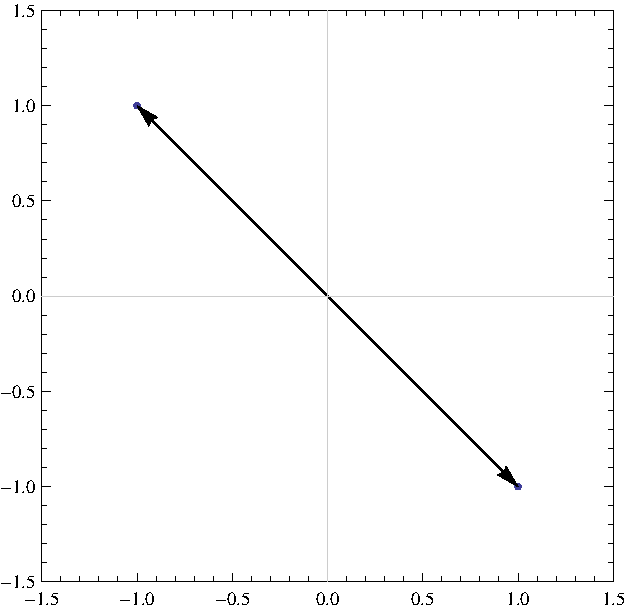
\includegraphics[ width = 2in ]{pdf/post_mortem/2d_before} \qquad
   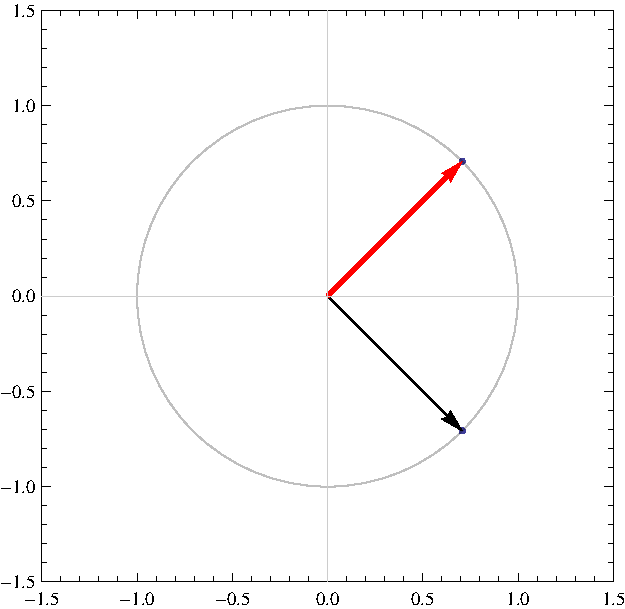
\includegraphics[ width = 2in ]{pdf/post_mortem/2d_after} 
   \caption{The row space before and after the SVD. The row vectors of the target matrix are on the left and the orthonormal resolution of the domain on the right. The null vector which completes the space is shown in red.}
   \label{fig:2d}
\end{figure}

\begin{figure}[htbp] %  figure placement: here, top, bottom, or page
   \centering
   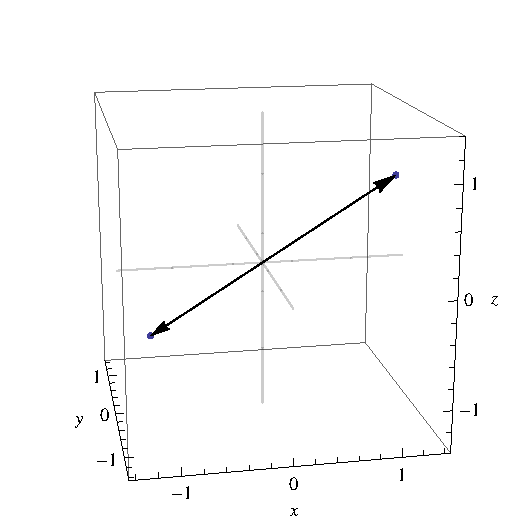
\includegraphics[ width = 2.2in ]{pdf/post_mortem/3d_before} \qquad
   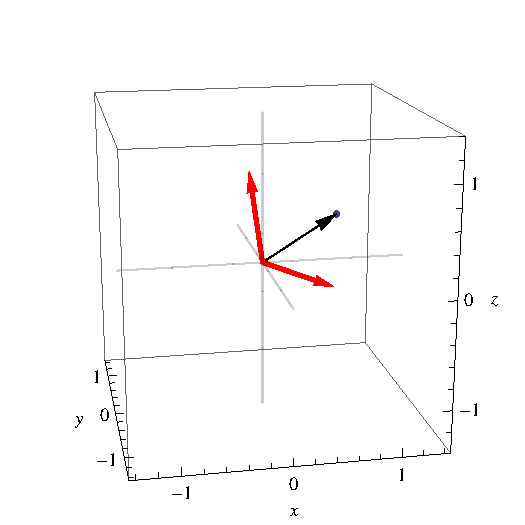
\includegraphics[ width = 2.2in ]{pdf/post_mortem/3d_after} 
   \caption{The column space before and after the SVD. Here too the column space is redundant and incomplete as seen by plotting the column vectors on the left. The orthonormal basis for the complete space is shown on the right.}
   \label{fig:3d}
\end{figure}

%%
\section{The action of the pseudoinverse}
Let's briefly touch on the issue raised in \S\eqref{sec:pi} and look at the product of a matrix and its pseudoinverse. The matrix products are these:

\begin{equation}
  \begin{array}{rcrrcl}
    \leftinv  &=& \Aexample & \Aplus &=& \rthree
    \mat{rrr}
    { 1 & 0 &  1\\
     -1 & \phantom{-}1 & -1\\
      1 & 0 &  1},\\
    \rightinv &=& \Aplus & \Aexample &=& \rtwo
    \mat{rr}
    { 1 & -1\\
     -1 & 1}.\\
  \end{array}
\end{equation}

We will look at another example in \S\eqref{lrfirst} and analyze the situation in the section on chiral inverses \S\eqref{sec:chiral} which will lead to the interpretation in terms of fundamental projectors \S\eqref{sec:orthproj}.

%%
\section{Thin SVD}
Look at the action of the $\sig{}$ matrix holding the singular values. Because of the sabot, the singular values are protected from the null spaces and interact with only the ranges. In effect these paddings prevent the null spaces from contributing the value of the target matrix. It's clear that the null vectors play no role in reconstituting the matrix $\A{}$.

%%
\subsection{An example}
In this context, it makes sense to fashion a \index{thin SVD}\textit{thin SVD} which excludes the null space vectors and the sabot. The thin $\sig{}$ matrix reduces to an $\by{\rho}{\rho}$ diagonal matrix. Using a tilde to denote the thin versions of the product matrices, the thin SVD for the matrix $\A{}$ becomes
\begin{equation}
  \begin{split}
    \A{} &= \svdthin{T},\\
    \Aexample & = \sthree \mat{r}{1\\-1\\1}\mat{c}{\sqrt{6}}\stwo\mat{cc}{1&-1}.
  \end{split}
  \label{eq:thin}
\end{equation}
The dimensions reductions for this problem are these:
$$
\begin{array}{lll}
\text{full SVD} & \svdax{T} & \by{3}{2} = \paren{\by{3}{3}}\paren{\by{3}{2}}\paren{\by{2}{2}} \\
\text{thin SVD} & \A{} = \svdthin{T} & \by{3}{2} = \paren{\by{3}{1}}\paren{\by{1}{1}}\paren{\by{1}{2}} \\
\end{array}
$$

Figure \eqref{fig:thin} displays the SVD before and after losing the null space vectors. Correlate this diagram to equation \eqref{eq:thin}.
\begin{figure}[htbp] %  figure placement: here, top, bottom, or page
   \centering
   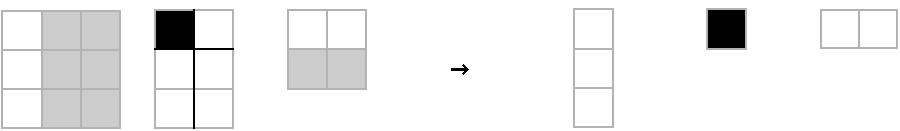
\includegraphics[ width = 5in ]{pdf/post_mortem/thin} 
   \caption{The secret to a thin SVD - lose the null spaces and the sabot. Matrices with incomplete row or column spaces are the only matrices that will shrink under the thin SVD.}
   \label{fig:thin}
\end{figure}

%%
\subsection{The general case}
As you might surmise, the dimensions and rank of the target matrix fully specify the dimensions for both the SVD and the thin SVD. The difference is the null space vectors; the lower the rank the thinner the ``thin SVD''. For a matrix 
\begin{equation}
  \A{}\in \mathbb{C}^{\by{m}{n}}_{\rho}
\end{equation}
the dimensions are given below in table \eqref{tab:bounty:thinsvd}.

\begin{table}[htdp]
\begin{center}
\begin{tabular}{llll}
SVD\quad & formulation & dimensions & size is rank\dots \\\hline
full & $\svd{*}$ & $\by{m}{n} = \paren{\by{m}{m}}\,\paren{\by{m}{n}}\,\paren{\by{n}{n}}$ & independent \\
thin & $\svdthin{*}$ & $\by{m}{n} = \paren{\by{m}{\rho}}\,\paren{\by{\rho}{\rho}}\,\paren{\by{\rho}{n}}$ & dependent \\[10pt]
\end{tabular}
\end{center}
\label{tab:bounty:thinsvd}
\caption{A comparison between the sizes of the component matrices for a full and thin SVD. Essentially, the thin SVD omits the null space vectors.}
\end{table}%

\endinput
\section{Exercises}
\begin{enumerate}
\item Consider the SVD given for $\Arrr{2}{2}{2}$:
\begin{equation*}
  \svdax{T} = 
  \mat{c|c}{y_{11} & y_{12} \\ y_{21} & y_{22}}
  \mat{cc}{\sigma_{1} & 0 \\ 0 & \sigma_{1}}
  \mat{cc}{x_{11} & x_{12} \\\hline x_{21} & x_{22}}.
\end{equation*}
Show by direct computation of the product that
\begin{equation*}
\begin{split}
  \A{} 
  &= \mat{cc}{
  \sigma_{1} x_{11} y_{11} + \sigma_{2} x_{12} y_{12} & \sigma_{1} x_{21} y_{11} + \sigma_{2} x_{22} y_{12} \\
  \sigma_{1} x_{11} y_{12} + \sigma_{2} x_{12} y_{22} & \sigma_{1} x_{21} y_{12} + \sigma_{2} x_{22} y_{22} } \\
  &= \sigma_{1} \mat{cc}{
  y_{11} \mat{cc}{x_{11} & x_{21}} \\
  y_{12} \mat{cc}{x_{11} & x_{21}}}
  + \sigma_{2} \mat{cc}{
  y_{21} \mat{cc}{x_{12} & x_{22}} \\
  y_{22} \mat{cc}{x_{12} & x_{22}}} \\
  &= \sigma_{1} y_{1}x_{1}^{T} + \sigma_{2} y_{2}x_{2}^{T}.
\end{split}
\end{equation*}
\item
\item
\end{enumerate}


\endinput

\endinput